%%=============================================================================
%% LaTeX sjabloon voor bachelorproef, HoGent Bedrijf en Organisatie
%% Opleiding Toegepaste Informatica
%%=============================================================================

\documentclass[fleqn,a4paper,12pt]{book}

%%=============================================================================
%% LaTeX sjabloon voor de bachelorproef, HoGent Bedrijf en Organisatie
%% Opleiding toegepaste informatica
%%
%% Structuur en algemene vormgeving. Meestal hoef je hier niets te wijzigen.
%%
%% Vormgeving gebaseerd op "The Legrand Orange Book", version 2.0 (9/2/15)
%% door Mathias Legrand (legrand.mathias@gmail.com) met aanpassingen door
%% Vel (vel@latextemplates.com). Het oorspronkelijke template is te vinden op
%% http://www.LaTeXTemplates.com
%%
%% Aanpassingen voor HoGent toegepaste informatica: 
%%   Bert Van Vreckem <bert.vanvreckem@hogent.be>
%% Licentie: 
%%   CC BY-NC-SA 3.0 (http://creativecommons.org/licenses/by-nc-sa/3.0/)
%%=============================================================================

%%-----------------------------------------------------------------------------
%% Packages
%%-----------------------------------------------------------------------------

\usepackage[top=3cm,bottom=3cm,left=3cm,right=3cm,headsep=10pt,a4paper]{geometry} % Page margins
\usepackage[utf8]{inputenc}  % Accenten gebruiken in tekst (vb. é ipv \'e)
\usepackage{amsfonts}        % AMS math packages: extra wiskundige
\usepackage{amsmath}         %   symbolen (o.a. getallen-
\usepackage{amssymb}         %   verzamelingen N, R, Z, Q, etc.)
\usepackage[english,dutch]{babel}    % Taalinstellingen: woordsplitsingen,
                             %  commando's voor speciale karakters
                             %  ("dutch" voor NL)
\usepackage{epigraph}
\usepackage{iflang}
\usepackage{eurosym}         % Euro-symbool €
\usepackage{geometry}
\usepackage{graphicx}        % Invoegen van tekeningen
\graphicspath{{img/}}       % Specifies the directory where pictures are stored
\usepackage{tikz}            % Required for drawing custom shapes
\usepackage[pdftex,bookmarks=true]{hyperref}
                             % PDF krijgt klikbare links & verwijzingen,
                             %  inhoudstafel
\usepackage{enumitem}        % Customize lists
\setlist{nolistsep}         % Reduce spacing between list items
\usepackage{listings}        % Broncode mooi opmaken
\usepackage{multirow}        % Tekst over verschillende cellen in tabellen
\usepackage{rotating}        % Tabellen en figuren roteren

\usepackage{booktabs}        % Required for nicer horizontal rules in tables

\usepackage{xcolor}          % Required for specifying colors by name
\definecolor{maincolor}{RGB}{0,147,208} % Define the main color used for 
                             % highlighting throughout the book
                             % 0, 147, 208 = officiële kleur HoGent FBO

% Paragraph style: no indent, add space between paragraphs
\setlength{\parindent}{0em}
\setlength{\parskip}{1em}

\usepackage{etoolbox}
\usepackage{titling} % Macros for title, author, etc
\usepackage{lipsum}          % Voor vultekst (lorem ipsum)

%----------------------------------------------------------------------------------------
%	FONTS
%----------------------------------------------------------------------------------------

\usepackage{avant} % Use the Avantgarde font for headings
%\usepackage{times} % Use the Times font for headings
\usepackage{mathptmx} % Use the Adobe Times Roman as the default text font together with math symbols from the Sym­bol, Chancery and Com­puter Modern fonts

\usepackage{microtype} % Slightly tweak font spacing for aesthetics
\usepackage[utf8]{inputenc} % Required for including letters with accents
\usepackage[T1]{fontenc} % Use 8-bit encoding that has 256 glyphs
\usepackage{longtable}
%------------------------------------------------------------------------------
%	TITLE PAGE
%------------------------------------------------------------------------------

\newcommand{\inserttitlepage}{%
\begin{titlepage}
  \newgeometry{top=2cm,bottom=1.5cm,left=1.5cm,right=1.5cm}
  \begin{center}

    \begingroup
    \rmfamily
    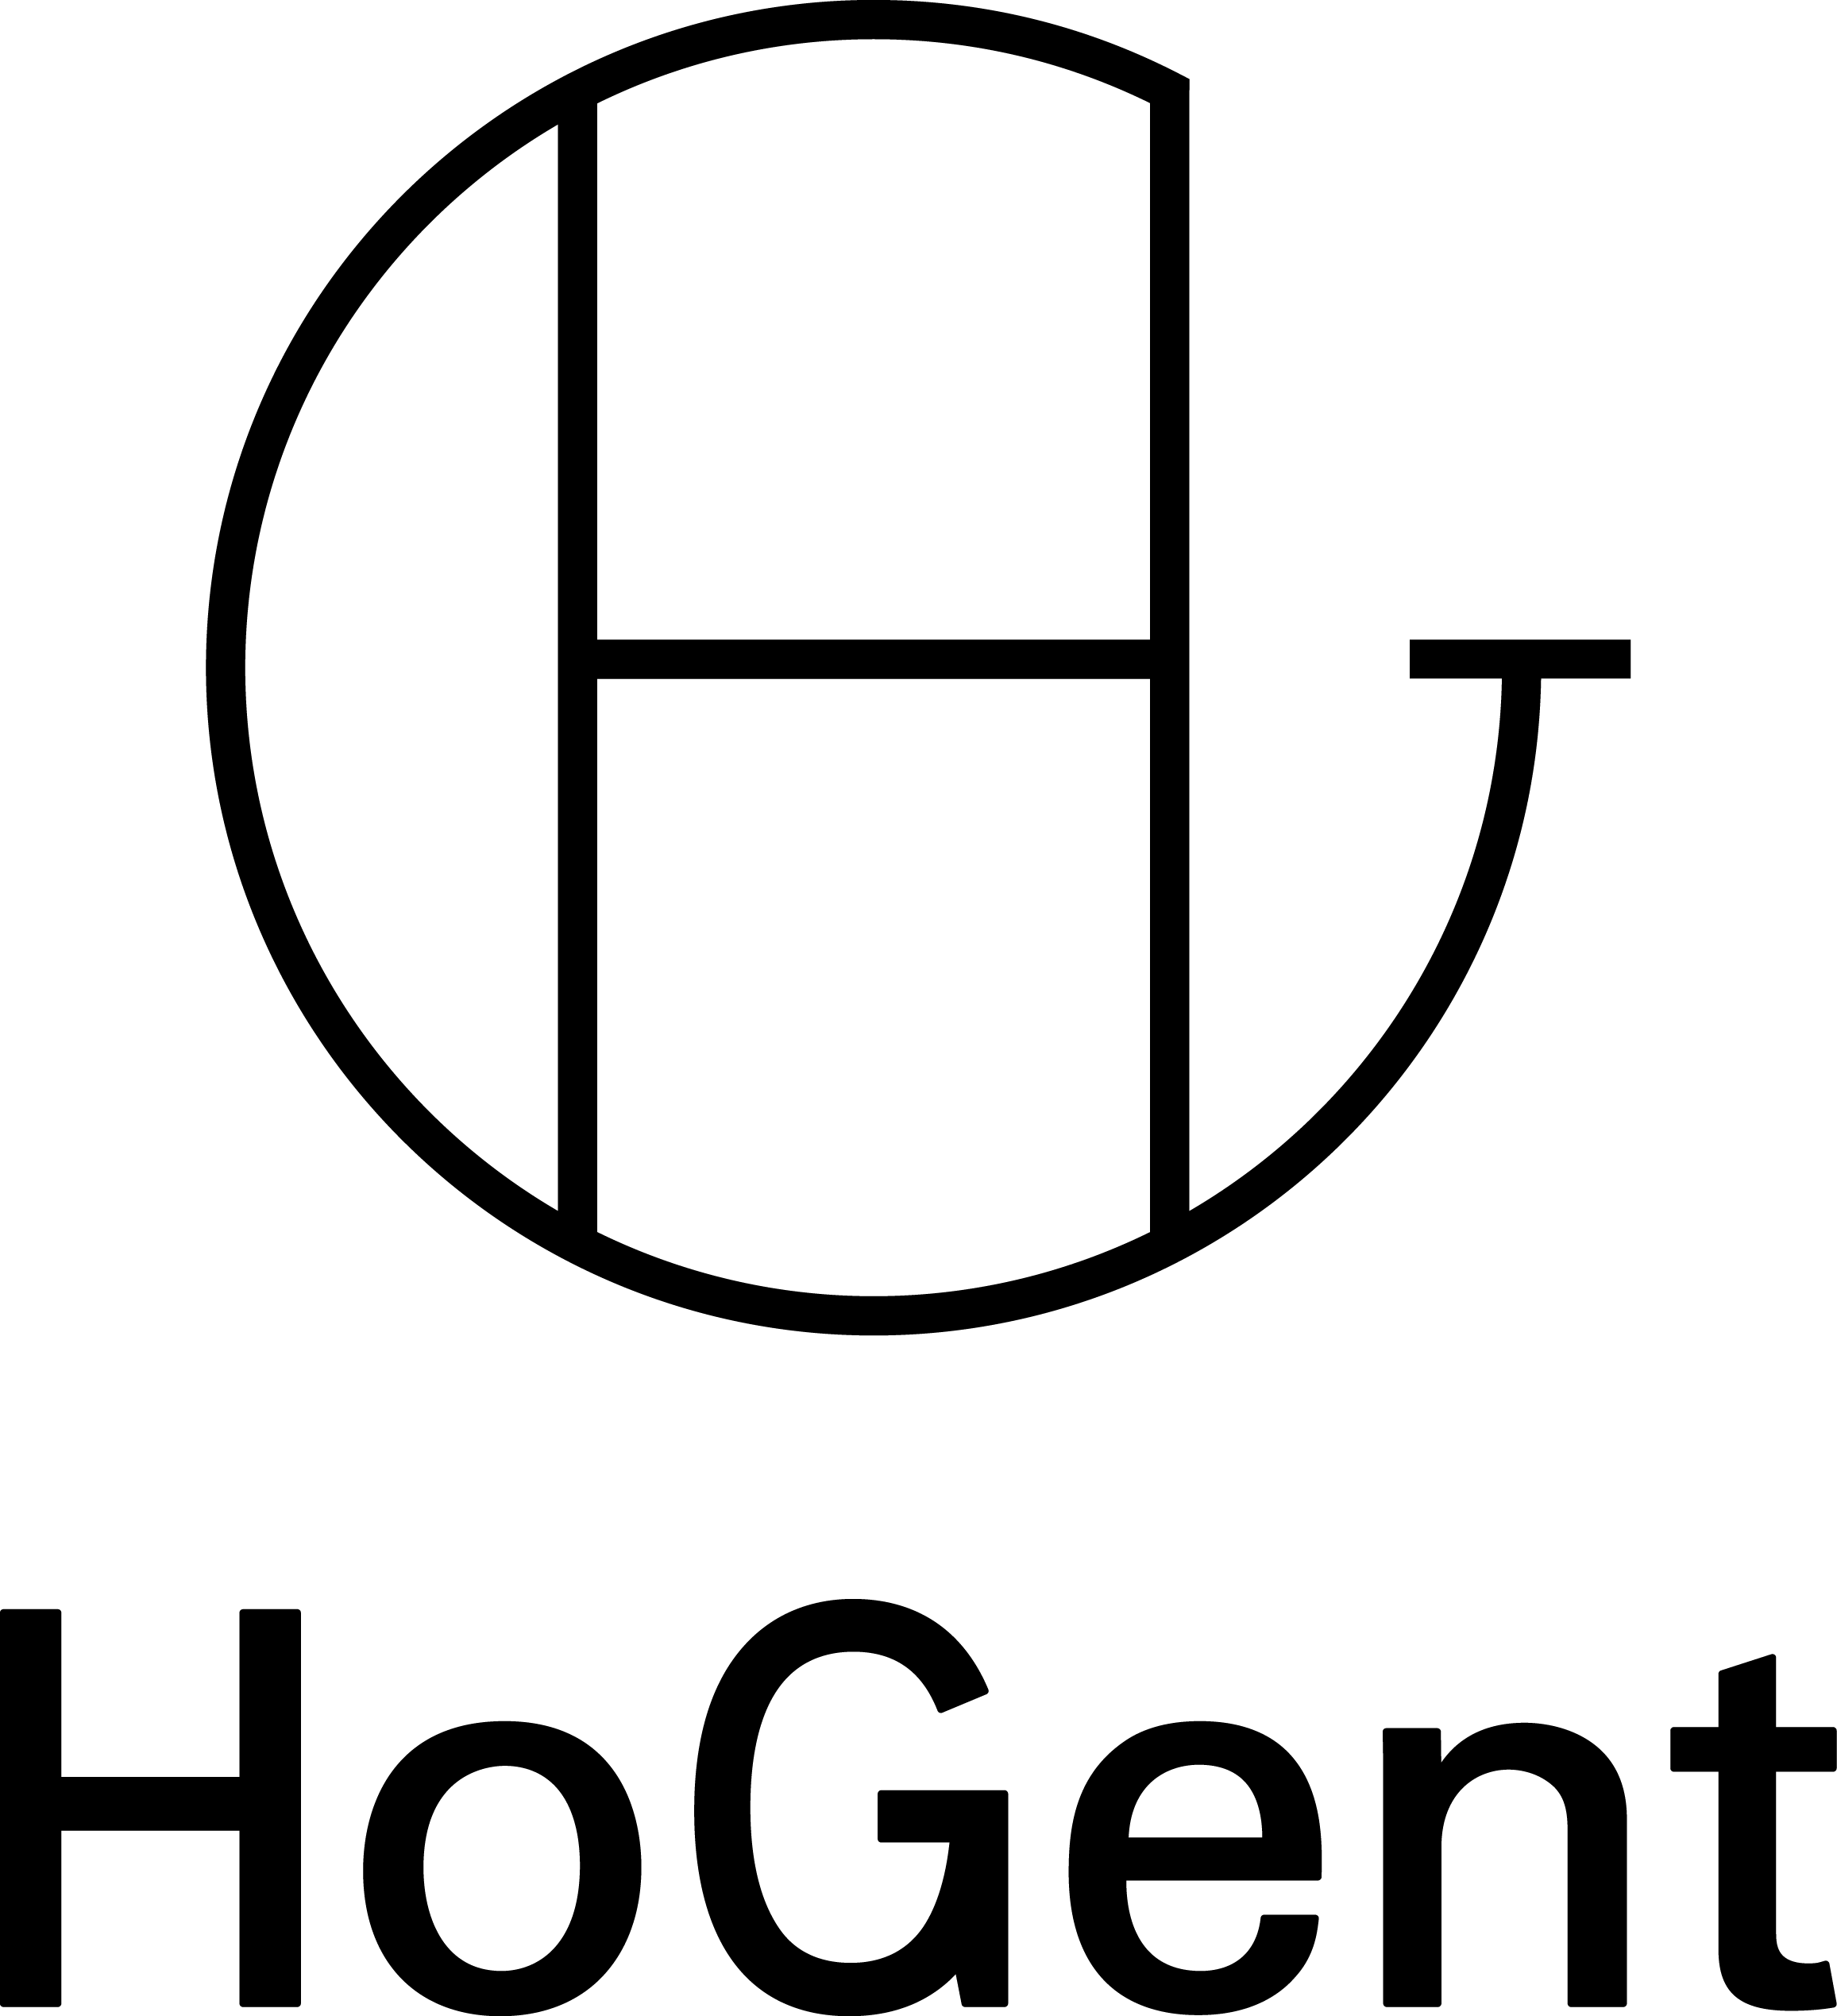
\includegraphics[width=2.5cm]{img/HG-beeldmerk-woordmerk}\\[.5cm]
    Faculteit Bedrijf en Organisatie\\[3cm]
    \titel
    \vfill
    \student\\[3.5cm]
    Scriptie voorgedragen tot het bekomen van de graad van\\professionele bachelor in de toegepaste informatica\\[2cm]
    Promotor:\\
    \promotor\\
    \ifdefempty{\copromotor}{\vspace{2.5cm}}{Co-promotor:\\\copromotor\\[2.5cm]}
    Instelling: \instelling\\[.5cm]
    Academiejaar: \academiejaar\\[.5cm]
    \ifcase \examenperiode \or Eerste \or Tweede \else Derde \fi examenperiode
    \endgroup

  \end{center}
  \restoregeometry
\end{titlepage}
  \emptypage
\begin{titlepage}
  \newgeometry{top=5.35cm,bottom=1.5cm,left=1.5cm,right=1.5cm}
  \begin{center}

    \begingroup
    \rmfamily
    \IfLanguageName{dutch}{Faculteit Bedrijf en Organisatie}{Faculty of Business and Information Management}\\[3cm]
    \titel
    \vfill
    \student\\[3.5cm]
    \IfLanguageName{dutch}{Scriptie voorgedragen tot het bekomen van de graad van\\professionele bachelor in de toegepaste informatica}{Thesis submitted in partial fulfilment of the requirements for the degree of\\professional bachelor of applied computer science}\\[2cm]
    Promotor:\\
    \promotor\\
    \ifdefempty{\copromotor}{\vspace{2.5cm}}{Co-promotor:\\\copromotor\\[2.5cm]}
    \IfLanguageName{dutch}{Instelling}{Institution}: \instelling\\[.5cm]
    \IfLanguageName{dutch}{Academiejaar}{Academic year}: \academiejaar\\[.5cm]
    \IfLanguageName{dutch}{%
    \ifcase \examenperiode \or Eerste \or Tweede \else Derde \fi examenperiode}{%
    \ifcase \examenperiode \or First \or Second \else Third \fi examination period}
    \endgroup

  \end{center}
  \restoregeometry
\end{titlepage}
}

%----------------------------------------------------------------------------------------
%	BIBLIOGRAPHY AND INDEX
%----------------------------------------------------------------------------------------

\usepackage[style=apa,backend=biber]{biblatex}
\usepackage{csquotes}
\DeclareLanguageMapping{dutch}{dutch-apa}
\addbibresource{bachproef-tin.bib} % BibTeX bibliography file
\addbibresource{../voorstel/voorstel.bib}
\defbibheading{bibempty}{}

\usepackage{calc} % For simpler calculation - used for spacing the index letter headings correctly
\usepackage{makeidx} % Required to make an index
\makeindex % Tells LaTeX to create the files required for indexing

%----------------------------------------------------------------------------------------
%	MAIN TABLE OF CONTENTS
%----------------------------------------------------------------------------------------

\usepackage{titletoc} % Required for manipulating the table of contents

\contentsmargin{0cm} % Removes the default margin

% Part text styling
\titlecontents{part}[0cm]
{\addvspace{20pt}\centering\large\bfseries}
{}
{}
{}

% Chapter text styling
\titlecontents{chapter}[1.25cm] % Indentation
{\addvspace{12pt}\large\sffamily\bfseries} % Spacing and font options for chapters
{\color{maincolor!60}\contentslabel[\Large\thecontentslabel]{1.25cm}\color{maincolor}} % Chapter number
{\color{maincolor}}
{\color{maincolor!60}\normalsize\;\titlerule*[.5pc]{.}\;\thecontentspage} % Page number

% Section text styling
\titlecontents{section}[1.25cm] % Indentation
{\addvspace{3pt}\sffamily\bfseries} % Spacing and font options for sections
{\contentslabel[\thecontentslabel]{1.25cm}} % Section number
{}
{\hfill\color{black}\thecontentspage} % Page number
[]

% Subsection text styling
\titlecontents{subsection}[1.25cm] % Indentation
{\addvspace{1pt}\sffamily\small} % Spacing and font options for subsections
{\contentslabel[\thecontentslabel]{1.25cm}} % Subsection number
{}
{\ \titlerule*[.5pc]{.}\;\thecontentspage} % Page number
[]

% List of figures
\titlecontents{figure}[0em]
{\addvspace{-5pt}\sffamily}
{\thecontentslabel\hspace*{1em}}
{}
{\ \titlerule*[.5pc]{.}\;\thecontentspage}
[]

% List of tables
\titlecontents{table}[0em]
{\addvspace{-5pt}\sffamily}
{\thecontentslabel\hspace*{1em}}
{}
{\ \titlerule*[.5pc]{.}\;\thecontentspage}
[]

%----------------------------------------------------------------------------------------
%	MINI TABLE OF CONTENTS IN PART HEADS
%----------------------------------------------------------------------------------------

% Chapter text styling
\titlecontents{lchapter}[0em] % Indenting
{\addvspace{15pt}\large\sffamily\bfseries} % Spacing and font options for chapters
{\color{maincolor}\contentslabel[\Large\thecontentslabel]{1.25cm}\color{maincolor}} % Chapter number
{}
{\color{maincolor}\normalsize\sffamily\bfseries\;\titlerule*[.5pc]{.}\;\thecontentspage} % Page number

% Section text styling
\titlecontents{lsection}[0em] % Indenting
{\sffamily\small} % Spacing and font options for sections
{\contentslabel[\thecontentslabel]{1.25cm}} % Section number
{}
{}

% Subsection text styling
\titlecontents{lsubsection}[.5em] % Indentation
{\normalfont\footnotesize\sffamily} % Font settings
{}
{}
{}

%----------------------------------------------------------------------------------------
%	PAGE HEADERS
%----------------------------------------------------------------------------------------

\usepackage{fancyhdr} % Required for header and footer configuration

\pagestyle{fancy}
\renewcommand{\chaptermark}[1]{\markboth{\sffamily\normalsize\bfseries\chaptername\ \thechapter.\ #1}{}} % Chapter text font settings
\renewcommand{\sectionmark}[1]{\markright{\sffamily\normalsize\thesection\hspace{5pt}#1}{}} % Section text font settings
\fancyhf{} \fancyhead[LE,RO]{\sffamily\normalsize\thepage} % Font setting for the page number in the header
\fancyhead[LO]{\rightmark} % Print the nearest section name on the left side of odd pages
\fancyhead[RE]{\leftmark} % Print the current chapter name on the right side of even pages
\renewcommand{\headrulewidth}{0.5pt} % Width of the rule under the header
\addtolength{\headheight}{2.5pt} % Increase the spacing around the header slightly
\renewcommand{\footrulewidth}{0pt} % Removes the rule in the footer
\fancypagestyle{plain}{\fancyhead{}\renewcommand{\headrulewidth}{0pt}} % Style for when a plain pagestyle is specified

% Removes the header from odd empty pages at the end of chapters
\makeatletter
\renewcommand{\cleardoublepage}{
\clearpage\ifodd\c@page\else
\hbox{}
\vspace*{\fill}
\thispagestyle{empty}
\newpage
\fi}

%----------------------------------------------------------------------------------------
%	THEOREM STYLES
%----------------------------------------------------------------------------------------

\usepackage{amsmath,amsfonts,amssymb,amsthm} % For math equations, theorems, symbols, etc

\newcommand{\intoo}[2]{\mathopen{]}#1\,;#2\mathclose{[}}
\newcommand{\ud}{\mathop{\mathrm{{}d}}\mathopen{}}
\newcommand{\intff}[2]{\mathopen{[}#1\,;#2\mathclose{]}}
\newtheorem{notation}{Notation}[chapter]

% Boxed/framed environments
\newtheoremstyle{maincolornumbox}% % Theorem style name
{0pt}% Space above
{0pt}% Space below
{\normalfont}% % Body font
{}% Indent amount
{\small\bf\sffamily\color{maincolor}}% % Theorem head font
{\;}% Punctuation after theorem head
{0.25em}% Space after theorem head
{\small\sffamily\color{maincolor}\thmname{#1}\nobreakspace\thmnumber{\@ifnotempty{#1}{}\@upn{#2}}% Theorem text (e.g. Theorem 2.1)
\thmnote{\nobreakspace\the\thm@notefont\sffamily\bfseries\color{black}---\nobreakspace#3.}} % Optional theorem note
\renewcommand{\qedsymbol}{$\blacksquare$}% Optional qed square

\newtheoremstyle{blacknumex}% Theorem style name
{5pt}% Space above
{5pt}% Space below
{\normalfont}% Body font
{} % Indent amount
{\small\bf\sffamily}% Theorem head font
{\;}% Punctuation after theorem head
{0.25em}% Space after theorem head
{\small\sffamily{\tiny\ensuremath{\blacksquare}}\nobreakspace\thmname{#1}\nobreakspace\thmnumber{\@ifnotempty{#1}{}\@upn{#2}}% Theorem text (e.g. Theorem 2.1)
\thmnote{\nobreakspace\the\thm@notefont\sffamily\bfseries---\nobreakspace#3.}}% Optional theorem note

\newtheoremstyle{blacknumbox} % Theorem style name
{0pt}% Space above
{0pt}% Space below
{\normalfont}% Body font
{}% Indent amount
{\small\bf\sffamily}% Theorem head font
{\;}% Punctuation after theorem head
{0.25em}% Space after theorem head
{\small\sffamily\thmname{#1}\nobreakspace\thmnumber{\@ifnotempty{#1}{}\@upn{#2}}% Theorem text (e.g. Theorem 2.1)
\thmnote{\nobreakspace\the\thm@notefont\sffamily\bfseries---\nobreakspace#3.}}% Optional theorem note

% Non-boxed/non-framed environments
\newtheoremstyle{maincolornum}% % Theorem style name
{5pt}% Space above
{5pt}% Space below
{\normalfont}% % Body font
{}% Indent amount
{\small\bf\sffamily\color{maincolor}}% % Theorem head font
{\;}% Punctuation after theorem head
{0.25em}% Space after theorem head
{\small\sffamily\color{maincolor}\thmname{#1}\nobreakspace\thmnumber{\@ifnotempty{#1}{}\@upn{#2}}% Theorem text (e.g. Theorem 2.1)
\thmnote{\nobreakspace\the\thm@notefont\sffamily\bfseries\color{black}---\nobreakspace#3.}} % Optional theorem note
\renewcommand{\qedsymbol}{$\blacksquare$}% Optional qed square
\makeatother

% Defines the theorem text style for each type of theorem to one of the three styles above
\newcounter{dummy}
\numberwithin{dummy}{section}
\theoremstyle{maincolornumbox}
\newtheorem{theoremeT}[dummy]{Theorem}
\newtheorem{problem}{Problem}[chapter]
\newtheorem{exerciseT}{Exercise}[chapter]
\theoremstyle{blacknumex}
\newtheorem{exampleT}{Example}[chapter]
\theoremstyle{blacknumbox}
\newtheorem{vocabulary}{Vocabulary}[chapter]
\newtheorem{definitionT}{Definition}[section]
\newtheorem{corollaryT}[dummy]{Corollary}
\theoremstyle{maincolornum}
\newtheorem{proposition}[dummy]{Proposition}

%----------------------------------------------------------------------------------------
%	DEFINITION OF COLORED BOXES
%----------------------------------------------------------------------------------------

\RequirePackage[framemethod=default]{mdframed} % Required for creating the theorem, definition, exercise and corollary boxes

% Theorem box
\newmdenv[skipabove=7pt,
skipbelow=7pt,
backgroundcolor=black!5,
linecolor=maincolor,
innerleftmargin=5pt,
innerrightmargin=5pt,
innertopmargin=5pt,
leftmargin=0cm,
rightmargin=0cm,
innerbottommargin=5pt]{tBox}

% Exercise box
\newmdenv[skipabove=7pt,
skipbelow=7pt,
rightline=false,
leftline=true,
topline=false,
bottomline=false,
backgroundcolor=maincolor!10,
linecolor=maincolor,
innerleftmargin=5pt,
innerrightmargin=5pt,
innertopmargin=5pt,
innerbottommargin=5pt,
leftmargin=0cm,
rightmargin=0cm,
linewidth=4pt]{eBox}

% Definition box
\newmdenv[skipabove=7pt,
skipbelow=7pt,
rightline=false,
leftline=true,
topline=false,
bottomline=false,
linecolor=maincolor,
innerleftmargin=5pt,
innerrightmargin=5pt,
innertopmargin=0pt,
leftmargin=0cm,
rightmargin=0cm,
linewidth=4pt,
innerbottommargin=0pt]{dBox}

% Corollary box
\newmdenv[skipabove=7pt,
skipbelow=7pt,
rightline=false,
leftline=true,
topline=false,
bottomline=false,
linecolor=gray,
backgroundcolor=black!5,
innerleftmargin=5pt,
innerrightmargin=5pt,
innertopmargin=5pt,
leftmargin=0cm,
rightmargin=0cm,
linewidth=4pt,
innerbottommargin=5pt]{cBox}

% Creates an environment for each type of theorem and assigns it a theorem text style from the "Theorem Styles" section above and a colored box from above
\newenvironment{theorem}{\begin{tBox}\begin{theoremeT}}{\end{theoremeT}\end{tBox}}
\newenvironment{exercise}{\begin{eBox}\begin{exerciseT}}{\hfill{\color{maincolor}\tiny\ensuremath{\blacksquare}}\end{exerciseT}\end{eBox}}
\newenvironment{definition}{\begin{dBox}\begin{definitionT}}{\end{definitionT}\end{dBox}}
\newenvironment{example}{\begin{exampleT}}{\hfill{\tiny\ensuremath{\blacksquare}}\end{exampleT}}
\newenvironment{corollary}{\begin{cBox}\begin{corollaryT}}{\end{corollaryT}\end{cBox}}

%----------------------------------------------------------------------------------------
%	REMARK ENVIRONMENT
%----------------------------------------------------------------------------------------

\newenvironment{remark}{\par\vspace{10pt}\small % Vertical white space above the remark and smaller font size
\begin{list}{}{
\leftmargin=35pt % Indentation on the left
\rightmargin=25pt}\item\ignorespaces % Indentation on the right
\makebox[-2.5pt]{\begin{tikzpicture}[overlay]
\node[draw=maincolor!60,line width=1pt,circle,fill=maincolor!25,font=\sffamily\bfseries,inner sep=2pt,outer sep=0pt] at (-15pt,0pt){\textcolor{maincolor}{R}};\end{tikzpicture}} % Orange R in a circle
\advance\baselineskip -1pt}{\end{list}\vskip5pt} % Tighter line spacing and white space after remark

%----------------------------------------------------------------------------------------
%	SECTION NUMBERING IN THE MARGIN
%----------------------------------------------------------------------------------------

\makeatletter
\renewcommand{\@seccntformat}[1]{\llap{\textcolor{maincolor}{\csname the#1\endcsname}\hspace{1em}}}
\renewcommand{\section}{\@startsection{section}{1}{\z@}
{-4ex \@plus -1ex \@minus -.4ex}
{1ex \@plus.2ex }
{\normalfont\large\sffamily\bfseries}}
\renewcommand{\subsection}{\@startsection {subsection}{2}{\z@}
{-3ex \@plus -0.1ex \@minus -.4ex}
{0.5ex \@plus.2ex }
{\normalfont\sffamily\bfseries}}
\renewcommand{\subsubsection}{\@startsection {subsubsection}{3}{\z@}
{-2ex \@plus -0.1ex \@minus -.2ex}
{.2ex \@plus.2ex }
{\normalfont\small\sffamily\bfseries}}
\renewcommand\paragraph{\@startsection{paragraph}{4}{\z@}
{-2ex \@plus-.2ex \@minus .2ex}
{.1ex}
{\normalfont\small\sffamily\bfseries}}

%----------------------------------------------------------------------------------------
%	PART HEADINGS
%----------------------------------------------------------------------------------------

% numbered part in the table of contents
\newcommand{\@mypartnumtocformat}[2]{%
\setlength\fboxsep{0pt}%
\noindent\colorbox{maincolor!20}{\strut\parbox[c][.7cm]{\ecart}{\color{maincolor!70}\Large\sffamily\bfseries\centering#1}}\hskip\esp\colorbox{maincolor!40}{\strut\parbox[c][.7cm]{\linewidth-\ecart-\esp}{\Large\sffamily\centering#2}}}%
%%%%%%%%%%%%%%%%%%%%%%%%%%%%%%%%%%
% unnumbered part in the table of contents
\newcommand{\@myparttocformat}[1]{%
\setlength\fboxsep{0pt}%
\noindent\colorbox{maincolor!40}{\strut\parbox[c][.7cm]{\linewidth}{\Large\sffamily\centering#1}}}%
%%%%%%%%%%%%%%%%%%%%%%%%%%%%%%%%%%
\newlength\esp
\setlength\esp{4pt}
\newlength\ecart
\setlength\ecart{1.2cm-\esp}
\newcommand{\thepartimage}{}%
\newcommand{\partimage}[1]{\renewcommand{\thepartimage}{#1}}%
\def\@part[#1]#2{%
\ifnum \c@secnumdepth >-2\relax%
\refstepcounter{part}%
\addcontentsline{toc}{part}{\texorpdfstring{\protect\@mypartnumtocformat{\thepart}{#1}}{\partname~\thepart\ ---\ #1}}
\else%
\addcontentsline{toc}{part}{\texorpdfstring{\protect\@myparttocformat{#1}}{#1}}%
\fi%
\startcontents%
\markboth{}{}%
{\thispagestyle{empty}%
\begin{tikzpicture}[remember picture,overlay]%
\node at (current page.north west){\begin{tikzpicture}[remember picture,overlay]%
\fill[maincolor!20](0cm,0cm) rectangle (\paperwidth,-\paperheight);
\node[anchor=north] at (4cm,-3.25cm){\color{maincolor!40}\fontsize{220}{100}\sffamily\bfseries\@Roman\c@part};
\node[anchor=south east] at (\paperwidth-1cm,-\paperheight+1cm){\parbox[t][][t]{8.5cm}{
\printcontents{l}{0}{\setcounter{tocdepth}{1}}%
}};
\node[anchor=north east] at (\paperwidth-1.5cm,-3.25cm){\parbox[t][][t]{15cm}{\strut\raggedleft\color{white}\fontsize{30}{30}\sffamily\bfseries#2}};
\end{tikzpicture}};
\end{tikzpicture}}%
\@endpart}
\def\@spart#1{%
\startcontents%
\phantomsection
{\thispagestyle{empty}%
\begin{tikzpicture}[remember picture,overlay]%
\node at (current page.north west){\begin{tikzpicture}[remember picture,overlay]%
\fill[maincolor!20](0cm,0cm) rectangle (\paperwidth,-\paperheight);
\node[anchor=north east] at (\paperwidth-1.5cm,-3.25cm){\parbox[t][][t]{15cm}{\strut\raggedleft\color{white}\fontsize{30}{30}\sffamily\bfseries#1}};
\end{tikzpicture}};
\end{tikzpicture}}
\addcontentsline{toc}{part}{\texorpdfstring{%
\setlength\fboxsep{0pt}%
\noindent\protect\colorbox{maincolor!40}{\strut\protect\parbox[c][.7cm]{\linewidth}{\Large\sffamily\protect\centering #1\quad\mbox{}}}}{#1}}%
\@endpart}
\def\@endpart{\vfil\newpage
\if@twoside
\if@openright
\null
\thispagestyle{empty}%
\newpage
\fi
\fi
\if@tempswa
\twocolumn
\fi}

%----------------------------------------------------------------------------------------
%	CHAPTER HEADINGS
%----------------------------------------------------------------------------------------

% A switch to conditionally include a picture, implemented by  Christian Hupfer
\newif\ifusechapterimage
\usechapterimagetrue
\newcommand{\thechapterimage}{}%
\newcommand{\chapterimage}[1]{\ifusechapterimage\renewcommand{\thechapterimage}{#1}\fi}%
\def\@makechapterhead#1{%
{\parindent \z@ \raggedright \normalfont
\ifnum \c@secnumdepth >\m@ne
\if@mainmatter
\begin{tikzpicture}[remember picture,overlay]
\node at (current page.north west)
{\begin{tikzpicture}[remember picture,overlay]
\node[anchor=north west,inner sep=0pt] at (0,0) {\ifusechapterimage\includegraphics[width=\paperwidth]{\thechapterimage}\fi};
\draw[anchor=west] (\Gm@lmargin,-9cm) node [line width=2pt,rounded corners=15pt,draw=maincolor,fill=white,fill opacity=0.5,inner sep=15pt]{\strut\makebox[22cm]{}};
\draw[anchor=west] (\Gm@lmargin+.3cm,-9cm) node {\huge\sffamily\bfseries\color{black}\thechapter. #1\strut};
\end{tikzpicture}};
\end{tikzpicture}
\else
\begin{tikzpicture}[remember picture,overlay]
\node at (current page.north west)
{\begin{tikzpicture}[remember picture,overlay]
\node[anchor=north west,inner sep=0pt] at (0,0) {\ifusechapterimage\includegraphics[width=\paperwidth]{\thechapterimage}\fi};
\draw[anchor=west] (\Gm@lmargin,-9cm) node [line width=2pt,rounded corners=15pt,draw=maincolor,fill=white,fill opacity=0.5,inner sep=15pt]{\strut\makebox[22cm]{}};
\draw[anchor=west] (\Gm@lmargin+.3cm,-9cm) node {\huge\sffamily\bfseries\color{black}#1\strut};
\end{tikzpicture}};
\end{tikzpicture}
\fi\fi\par\vspace*{270\p@}}}

%-------------------------------------------

\def\@makeschapterhead#1{%
\begin{tikzpicture}[remember picture,overlay]
\node at (current page.north west)
{\begin{tikzpicture}[remember picture,overlay]
\node[anchor=north west,inner sep=0pt] at (0,0) {\ifusechapterimage\includegraphics[width=\paperwidth]{\thechapterimage}\fi};
\draw[anchor=west] (\Gm@lmargin,-9cm) node [line width=2pt,rounded corners=15pt,draw=maincolor,fill=white,fill opacity=0.5,inner sep=15pt]{\strut\makebox[22cm]{}};
\draw[anchor=west] (\Gm@lmargin+.3cm,-9cm) node {\huge\sffamily\bfseries\color{black}#1\strut};
\end{tikzpicture}};
\end{tikzpicture}
\par\vspace*{270\p@}}
\makeatother

%----------------------------------------------------------------------------------------
%	HYPERLINKS IN THE DOCUMENTS
%----------------------------------------------------------------------------------------

\usepackage{hyperref}
\hypersetup{hidelinks,backref=true,pagebackref=true,hyperindex=true,colorlinks=false,breaklinks=true,urlcolor= maincolor,bookmarks=true,bookmarksopen=false,pdftitle={Title},pdfauthor={Author}}
\usepackage{bookmark}
\bookmarksetup{
open,
numbered,
addtohook={%
\ifnum\bookmarkget{level}=0 % chapter
\bookmarksetup{bold}%
\fi
\ifnum\bookmarkget{level}=-1 % part
\bookmarksetup{color=maincolor,bold}%
\fi
}
}

%----------------------------------------------------------------------------------------
%	Java source code
%----------------------------------------------------------------------------------------

% Commando voor invoegen Java-broncodebestanden (dank aan Niels Corneille)
% Gebruik:
%   \codefragment{source/MijnKlasse.java}{Uitleg bij de code}
%
% Je kan dit aanpassen aan de taal die je zelf het meeste gebruikt in je
% bachelorproef.
\newcommand{\codefragment}[2]{ \lstset{%
  language=java,
  breaklines=true,
  float=th,
  caption={#2},
  basicstyle=\scriptsize,
  frame=single,
  extendedchars=\true
}
\lstinputlisting{#1}}

% Leeg blad
\newcommand{\emptypage}{%
\newpage
\thispagestyle{empty}
\mbox{}
\newpage
}


%%---------- Documenteigenschappen --------------------------------------------
%% TODO: Vul dit aan met je eigen info:

% Je eigen naam
\newcommand{\student}{Jorik Spiesschaert}

% De naam van je promotor (lector van de opleiding)
\newcommand{\promotor}{Stijn Lievens}

% De naam van je co-promotor. Als je promotor ook je opdrachtgever is en je
% dus ook inhoudelijk begeleidt (en enkel dan!), mag je dit leeg laten.
\newcommand{\copromotor}{Jochen Stroobants}

% Indien je bachelorproef in opdracht van/in samenwerking met een bedrijf of
% externe organisatie geschreven is, geef je hier de naam. Zoniet laat je dit
% zoals het is.
\newcommand{\instelling}{DHL Pharma-Logistics}

% De titel van het rapport/bachelorproef
\newcommand{\titel}{Een vergelijkende studie tussen Data Vault 2.0 en het dimensioneel model bij het modelleren van een datawarehouse.}

% Datum van indienen (gebruik telkens de deadline, ook al geef je eerder af)
\newcommand{\datum}{31 mei 2019}

% Academiejaar
\newcommand{\academiejaar}{2018-2019}

% Examenperiode
%  - 1e semester = 1e examenperiode => 1
%  - 2e semester = 2e examenperiode => 2
%  - tweede zit  = 3e examenperiode => 3
\newcommand{\examenperiode}{2}

%%=============================================================================
%% Inhoud document
%%=============================================================================

\begin{document}

%---------- Taalselectie ------------------------------------------------------
% Als je je bachelorproef in het Engels schrijft, haal dan onderstaande regel
% uit commentaar. Let op: de tekst op de voorkaft blijft in het Nederlands, en
% dat is ook de bedoeling!

%\selectlanguage{english}

%---------- Titelblad ---------------------------------------------------------
\inserttitlepage

%---------- Samenvatting, voorwoord -------------------------------------------
\usechapterimagefalse
%%=============================================================================
%% Voorwoord
%%=============================================================================

\chapter*{Woord vooraf}
\label{ch:voorwoord}

%% TODO:
%% Het voorwoord is het enige deel van de bachelorproef waar je vanuit je
%% eigen standpunt (``ik-vorm'') mag schrijven. Je kan hier bv. motiveren
%% waarom jij het onderwerp wil bespreken.
%% Vergeet ook niet te bedanken wie je geholpen/gesteund/... heeft

Voor het bekomen van een professionele bachelor in de Toegepaste Informatica dient een bachelorproef geschreven te worden. 

Het onderwerp van deze bachelorproef werd mij aangebracht door Jochen Stroobants bij de start van mijn stage. Als stageopdracht diende een data warehouse opgesteld te worden aan de hand van Data Vault 2.0. Zelf was ik kritisch tegenover deze keuze en ik vroeg mij dan ook af of Data Vault 2.0 de juiste keuze was ten opzichte van het dimensioneel model. Het leek mij zeer interessant om de vergelijking te maken tussen beide modellen en om te concluderen of het dimensioneel geen betere keuze was.

Graag bedank ik in eerste instantie mijn promotor Stijn Lievens voor de uitgebreide feedback die ik ontving tijdens het opstellen van een voorstel en tijdens het schrijven van deze paper. Door zijn kritische kijk kon ik de kwaliteit van deze paper naar een hoger niveau brengen. 

Anderzijds bedank ik graag het bedrijf Cubis Solutions, omdat ik gebruik kon en mocht maken van hun infrastructuur. In het bijzondere wil ik graag Jochen Stroobants, Sven Van Rillaer en Sander Allert bedanken voor hun kennis en feedback die ik ontving tijdens het opstellen van deze paper.
%%=============================================================================
%% Samenvatting
%%=============================================================================

% TODO: De "abstract" of samenvatting is een kernachtige (~ 1 blz. voor een
% thesis) synthese van het document.
%
% Deze aspecten moeten zeker aan bod komen:
% - Context: waarom is dit werk belangrijk?
% - Nood: waarom moest dit onderzocht worden?
% - Taak: wat heb je precies gedaan?
% - Object: wat staat in dit document geschreven?
% - Resultaat: wat was het resultaat?
% - Conclusie: wat is/zijn de belangrijkste conclusie(s)?
% - Perspectief: blijven er nog vragen open die in de toekomst nog kunnen
%    onderzocht worden? Wat is een mogelijk vervolg voor jouw onderzoek?
%
% LET OP! Een samenvatting is GEEN voorwoord!

%%---------- Nederlandse samenvatting -----------------------------------------
%
% TODO: Als je je bachelorproef in het Engels schrijft, moet je eerst een
% Nederlandse samenvatting invoegen. Haal daarvoor onderstaande code uit
% commentaar.
% Wie zijn bachelorproef in het Nederlands schrijft, kan dit negeren, de inhoud
% wordt niet in het document ingevoegd.

\IfLanguageName{english}{%
\selectlanguage{dutch}
\chapter*{Samenvatting}
\selectlanguage{english}
}{}

%%---------- Samenvatting -----------------------------------------------------
% De samenvatting in de hoofdtaal van het document

\chapter*{\IfLanguageName{dutch}{Samenvatting}{Abstract}}

DHL Pharma Logistics wil een data warehouse aanmaken om hun rapporteringen te automatiseren. Het data warehouse wordt gemodelleerd via de Data Vault 2.0 methodologie. In deze paper wordt onderzocht of modelleren via deze manier wel degelijk de juiste keuze was ten opzichte van het dimensioneel model. 

Vooraleer het onderzoek van start gaat, wordt een literatuurstudie weergegeven met de informatie en begrippen die nodig zijn om het volledige onderzoek mee te kunnen volgen.

Vervolgens wordt in het onderzoek twee data warehouses opgebouwd op basis van dezelfde data. Er zal een data warehouse gemodelleerd worden via Data Vault 2.0, de andere data warehouse zal gebaseerd zijn op het dimensioneel model.

Het vergelijkend onderzoek wordt uitgevoerd op basis van vijf pijlers: performantie, complexiteit, flexibiliteit, schaalbaarheid en audit. Zowel Data Vault 2.0 als het dimensioneel model worden onderworpen aan deze vijf pijlers, op basis van de noden van DHL Pharma Logistics wordt een juiste conclusie opgemaakt. 

Als resultaat in dit onderzoek blijkt dat het kiezen voor het opstellen van een data warehouse aan de hand van dimensioneel modelleren een betere keuze was geweest.

Naar de toekomst toe kan er onderzocht worden of Data Vault 2.0 een juiste keuze kan zijn bij het opstellen van big data modellen.

%---------- Inhoudstafel ------------------------------------------------------
\pagestyle{empty} % No headers
\tableofcontents % Print the table of contents itself
\cleardoublepage % Forces the first chapter to start on an odd page so it's on the right
\pagestyle{fancy} % Print headers again

%---------- Lijst figuren, afkortingen, ... -----------------------------------

% Indien gewenst kan je hier een lijst van figuren/tabellen opgeven. Geef in
% dat geval je figuren/tabellen altijd een korte beschrijving:
%
%  \caption[korte beschrijving]{uitgebreide beschrijving}

\listoffigures
\listoftables

% Als je een lijst van afkortingen of termen wil toevoegen, dan hoort die
% hier thuis. Gebruik bijvoorbeeld de ``glossaries'' package.
% https://www.sharelatex.com/learn/Glossaries

%%---------- Kern -------------------------------------------------------------

%%=============================================================================
%% Inleiding
%%=============================================================================

\chapter{Inleiding}
\label{ch:inleiding}
Beslissingen genomen door het management worden vaak ondersteund op basis van data en rapporteringen. Bij sommige bedrijven worden de benodigde data nog steeds manueel uitgerekend. Deze methodologie heeft enkele nadelen: kans op fouten, tijdrovend, ... Bedrijven die dit proces willen automatiseren en digitaliseren moeten hiervoor een data warehouse opbouwen. Data afkomstig uit verschillende bronnen worden dan ingeladen in één centrale plaats. Op basis van de data afkomstig uit een data warehouse kan een rapporteringsomgeving de data visualiseren, dashboards en rapporteringen opmaken. Het is gebruikelijk dat het datamodel in een data warehouse opgebouwd wordt aan de hand van een dimensioneel model. Dit kan ook gebeuren aan de hand van een ander model, genaamd Data Vault. 

Bij DHL Pharma Logistics wordt een data warehouse opgebouwd aan de hand van het Data Vault model. Maar waar zitten de verschillen bij Data Vault in vergelijking met het dimensioneel model? Was de keuze voor Data Vault bij het modelleren van de data warehouse juist voor DHL Pharma Logistics?



\section{Probleemstelling}
\label{sec:probleemstelling}

Wie interesse heeft in Business Intelligence of modelleren van data, is ongetwijfeld al in aanraking gekomen met het dimensioneel model. Maar dit is heus niet de enigste techniek die beschikbaar is voor het modelleren van datamodellen. Data Vault 2.0 werd al geïmplementeerd bij bedrijven zoals IBM, Oracle en ING. Wat zouden de redenen kunnen zijn waarom deze bedrijven kiezen voor Data Vault? Met welke elementen onderscheidt Data Vault zich ten opzichte van het dimensioneel model? Dit onderzoek is gericht naar BI consultants en alle belanghebbenden.

\section{Onderzoeksvraag}
\label{sec:onderzoeksvraag}
In dit onderzoek wordt een vergelijkende studie uitgevoerd tussen het dimensioneel modelleren en Data Vault 2.0, dit toegepast op een case bij DHL Pharma Logistics. Er wordt onderzocht waar de verschillen zitten bij het modelleren met Data Vault 2.0 en het dimensioneel modelleren. Er zal een antwoord trachten gevonden te worden op volgende deelvragen:

\begin{itemize}
	\item \textbf{Performantie:} is er een significant verschil tussen de performantie tussen beide modellen?
	\item \textbf{Audit:} hoe wordt er omgegaan met de traceerbaarheid in beide modellen?
	\item \textbf{Schaalbaarheid:} hoe wordt er omgegaan met grote volumes data?
	\item \textbf{Complexiteit:} zijn beide modellen makkelijk begrijpbaar (voor IT en business)?
	\item \textbf{Flexibiliteit:} hoe makkelijk kunnen wijzigingen/toevoegingen gemaakt worden in beide systemen?
	
\end{itemize}

\section{Onderzoeksdoelstelling}
\label{sec:onderzoeksdoelstelling}
DHL Pharma Logistics wil een data warehouse ontwerpen voor hun rapporteringen te kunnen automatiseren. De data warehouse zal gemodelleerd worden via Data Vault. De vraag is echter of dit een juiste beslissing was. De andere mogelijkheid was om de data warehouse te ontwerpen via het dimensioneel ontwerpen. 

\section{Opzet van deze bachelorproef}
\label{sec:opzet-bachelorproef}

% Het is gebruikelijk aan het einde van de inleiding een overzicht te
% geven van de opbouw van de rest van de tekst. Deze sectie bevat al een aanzet
% die je kan aanvullen/aanpassen in functie van je eigen tekst.

De rest van deze bachelorproef is als volgt opgebouwd:

In hoofdstuk~\ref{ch:stand-van-zaken} wordt een overzicht gegeven van de stand van zaken binnen het onderzoeksdomein, op basis van een literatuurstudie.

In hoofdstuk~\ref{ch:methodologie} wordt de methodologie toegelicht en worden de gebruikte onderzoekstechnieken besproken om een antwoord te kunnen formuleren op de onderzoeksvragen.

% TODO: Vul hier aan voor je eigen hoofstukken, één of twee zinnen per hoofdstuk

In Hoofdstuk~\ref{ch:conclusie}, tenslotte, wordt de conclusie gegeven en een antwoord geformuleerd op de onderzoeksvragen. Daarbij wordt ook een aanzet gegeven voor toekomstig onderzoek binnen dit domein.


\chapter{Stand van zaken}
\label{ch:stand-van-zaken}

% Tip: Begin elk hoofdstuk met een paragraaf inleiding die beschrijft hoe
% dit hoofdstuk past binnen het geheel van de bachelorproef. Geef in het
% bijzonder aan wat de link is met het vorige en volgende hoofdstuk.

% Pas na deze inleidende paragraaf komt de eerste sectiehoofding.

Dit hoofdstuk bevat een literatuurstudie omtrent data warehousing. Na het lezen van dit hoofdstuk zullen begrippen zoals dimensioneel modelleren, data vault 2.0 en data warehousing jou niet meer onbekend zijn en waarom er nood is aan data warehousing. Ook zullen beide modelleertechnieken dieper bekeken worden.

%\textcite{Knuth1998}
\section{Inleiding data warehousing}

\epigraph{Torture the data, and it will confess to anything. }{\textit{Ronald Coase \\ Winnaar Nobelprijs in Economie (1991)}}

Veel moderne, digitale bedrijven genereren tegenwoordig enorme volumes data. Deze data kan afkomstig zijn uit verschillende bronnen: CRM-systeem, flat-files (vb. rekenbladen), Twitter-feeds, ... Bestuursleden gebruiken data om beslissingen te nemen die de onderneming toelaat om te (blijven) groeien of om bepaalde problemen op te sporen. Stel dat een onderneming meer kosten maakt dan opbrengsten. Op basis van alle gegevens die het bedrijf bezit, kan hieruit dan een analyse gemaakt worden. Zijn er overbodige kosten? Worden onze producten/diensten aan een te lage prijs verkocht? Dit zijn maar enkele vragen die kunnen opgelost worden wanneer het bestuur de correcte rapporteringen ontvangt. 

\subsection{Soorten data}
Er kan een onderscheid gemaakt worden tussen verschillende soorten data. Voornamelijk kunnen we informatie opdelen in 2 categorieën: gestructureerde en ongestructureerde data. Volgens een artikel van ~\textcite{Langseth2005}, bestaat 95\% van de globale informatie uit ongestructureerde data. 

\subsubsection{Gestructureerde data}
Data afkomstig uit een relationele databank (RDBMS) is meestal gestructureerd. Deze data is meestal ingedeeld in categorieën, denk bijvoorbeeld maar aan postcode, naam, klantennummer, ... Hieruit volgt dat deze data heel gemakkelijk te doorzoeken is. 

\subsubsection{Ongestructureerde data}
Deze informatie kan niet gemakkelijk worden opgeslagen in databanken. Denk maar aan rekenbladen, emails, tweets, muziek, ... Data afkomstig uit IoT-apparaten zijn meestal ook ongestructureerd. Deze data bevat vaak ook heel nuttige informatie die organisaties graag willen benuttigen. Denk bijvoorbeeld maar aan tweets: hoe gelukkig zijn klanten over een bepaald product? Hoeveel mails worden er maandelijks ontvangen met klachten?

\subsection{Wat is een data warehouse?}
De definitie van een data warehouse luidt als volgt: \textit{"een subject-georiënteerde, geïntegreerde, tijd-variante, niet-vluchtige collectie van gegevens dat in eerste instantie gebruikt wordt bij organisaties om beslissingen te nemen"} ~\autocite{Panos2000}.

\paragraph{Subject-georiënteerd}
Dit begrip slaat op het feit dat een data warehouse met de reden gebouwd is om data te analyseren, niet om transacties op toe te passen. Dit wordt uitgebreid besproken in subsectie \ref{sec:oltp-vs-olap}.


\paragraph{Geïntegreerd}
Dit betekent dat de data warehouse een "centrale" databank is die gegevens bevat vanuit verschillende bronsystemen (bijvoorbeeld gegevens uit het klantenbestand en gegevens uit het verkoopsysteem). Deze data kan effectief ingeladen worden, maar ook opgeslagen worden in virtuele tabellen.

\paragraph{Tijd-variant}
Alle data van het verleden, moet terug te vinden zijn in de data warehouse. Dit betekent dat data uit het verleden (bijvoorbeeld een vorig adres van een klant) moet beschikbaar zijn, ook al is deze in het transactioneel systeem aangepast.

\paragraph{Niet-vluchtig}
De data die in het systeem zit, moet onveranderlijk zijn, ook al zijn deze fout. Om de foutieve data toch aan te passen, zal er een nieuwe rij moeten toegevoegd worden die de juiste data bevat, die een hogere versie bevat dan de vorige rij. 

\paragraph{Conclusie}
We kunnen dus uit de definitie van een data warehouse afleiden dat het een grote databron is die alle (gestructureerde en ongestructureerde (indien mogelijk)) gegevens bevat die een organisatie bezit vanaf het moment waarbij de data warehouse geïmplementeerd is tot het heden. Op deze databron worden dan analyses gemaakt.

\subsection{Waarom is er nood aan een data warehouse?}
Een organisatie heeft tegenwoordig heel wat data ter beschikking. Vaak is deze data gefragmenteerd over verschillende systemen. Wanneer men een analyse wil opmaken op basis van de verspreide data, zal dat niet evident zijn. 

Om deze reden wordt een data warehouse ontworpen. Hierin worden gegevens, verspreidt over meerdere bronnen, in één bron verzameld. Zo kunnen rapporteringen makkelijk en flexibel opgebouwd worden. 

Een andere reden voor het opbouwen van een data warehouse is dat je de historiek van alle data kan bijhouden. Wanneer er bijvoorbeeld gegevens aangepast zijn in het transactionele systeem, dan zijn de oude gegevens vaak moeilijk te achterhalen (omdat deze dat vaak overschreven wordt). Door verschillende versies bij te houden van entiteiten, kan je oudere data makkelijk opzoeken.

Wanneer men rapporteringen wil opvragen aan het transactionele systeem, vergt dit ook extra belasting van de server. Dit komt doordat het datamodel die opgebouwd werd niet geoptimaliseerd is om zware SELECT-queries af te handelen. Dit zou niet alleen de server meer belasten, bovendien zal dit ook zorgen voor een tragere rapportering. 


\subsection{Wat is het doel van een data warehouse?}
Het belangrijkste doel dat een data warehouse heeft is om een \textbf{correcte} rapportering op te leveren. Beslissingen in organisaties worden genomen op basis van rapporten.

\paragraph{Data kwaliteit}
Zoals eerder aangekaart, is het belangrijk dat rapporten de juiste gegevens bevat. Hieruit volgt dat data kwaliteit een heel belangrijk aspect is. Vaak zijn er verschillende oorzaken waarom de data kwaliteit niet voldoet:

\begin{itemize}
	\item Inconsistente data tussen verschillende systemen
	\item Incorrecte gegevens
	\item Onvoldoende validatie bij het invoeren van gegevens
	\item Onjuiste gegevensbewerkingen
	\item \ldots
\end{itemize}  
~\autocite{Helfert2002}

Gegevens die in een data warehouse geladen worden, ondergaan een proces (zie paragraaf \ref{sec:etl}). In dit proces wordt de data gemanipuleerd zodat de data kwaliteit verhoogd wordt.

\paragraph{Performantie}
We kunnen een onderscheid maken tussen 3 verschillende soorten beslissingen: operationele (dagelijks), tactische (jaarlijks) en strategische (lange termijn) beslissingen. Wanneer we operationele rapporten nodig hebben, verwachten we dan ook dat deze onmiddelijk kunnen opgeleverd worden. Het datamodel van een data warehouse wordt geoptimaliseerd voor het ophalen van data in plaats van het te kunnen stockeren. De data wordt 's nachts ingeladen zodat werknemers geen performantieproblemen hieromtrend ondervinden. 

\subparagraph{De toekomst}
Door de komst van in-memory databanken merken we op dat een deel van de (operationele) rapportering opnieuw verhuist naar de transactionele databanken. Dit heeft enerzijds te maken met de snelheid van de databanken en anderzijds met het feit dat queries om operationele rapporten op te vragen gebruikelijk niet zo belastend zijn. Zo kan er gewerkt worden met \textbf{live data} (doordat deze niet 's nachts moet ingeladen worden in de data warehouse). De voorwaarde hiervoor is dat alle benodigde data beschikbaar is binnen dat geïntegreerd systeem. Een voorbeeld van een in-memory databank is HANA, een technologie ontwikkelt door SAP.

\paragraph{Automatisering}
Doordat alle rapporteringsnoden geautomatiseerd kunnen worden, heeft dit natuurlijk als voordeel dat personeelsleden deze niet meer manueel hoeven te maken/berekenen. Zo kunnen ze hun tijd spenderen aan andere prioriteiten. Deze data kan dan worden voorgesteld in een overzichtelijke omgeving (zie sectie \ref{sec:omgeving}).

\subsection{Wat is OLTP en wat zijn de verschillen met OLAP?}
\label{sec:oltp-vs-olap}
On-line transactional processing (OLTP) systemen zijn voornamelijk klantgericht. Het datamodel is opgebouwd rond het efficiënt verwerken van transacties. On-line analytical processing (OLAP) systemen zijn martkgericht. De data in een OLAP-systemen worden gebruikt om analyses op uit te voeren ~\autocite{Satyanarayana2010}.


\paragraph{Inhoudelijk}
Bij OLAP systemen worden meta data opgeslagen bij de entiteiten. Voorbeelden hiervan zijn: tijdstip van inladen, van welke bron de data komt, ... Het grote voordeel hierbij is dat wanneer een fout gebeurt, er gemakkelijker kan achterhaalt worden waar het fout liep. Ook wordt de historische data ook bewaard, in tegenstelling tot OLTP. Bij OLTP wordt de te wijzigen data overschreven. Het gevolg hiervan is dat de volume data bij OLAP doorgaans groter zal zijn.

\paragraph{Toegankelijkheid}
Wanneer men data wil verkrijgen/wijzigen in een OLTP systeem, moet er rekening gehouden met een aantal aspecten. Een transactie in een OLTP omgeving moet voldoen aan enkele eisen:
\begin{itemize}
	\item \textbf{Atomic:} Wanneer een transactie afgebroken is, mag er niets gewijzigd zijn in de databank.
	\item \textbf{Consistent:} Als een deel van de transactie faalt, zullen alle doorgevoerde wijzigingen in die transactie ongedaan gemaakt worden en zal de databank terugkeren naar een consistente staat.
	\item \textbf{Isolated:} Transacties worden geïsoleerd, transacties mogen in geen enkel geval elkaar beïnvloeden.
	\item \textbf{Durable:} Wanneer een transactie is doorgevoerd, kan deze niet meer ongedaan gemaakt worden.
\end{itemize}  

Bij een OLAP-systeem worden geen transacties doorgevoerd, enkel leesopdrachten. Dat vermindert de complexiteit en verhoogt de snelheid van de queries ~\autocite{Satyanarayana2010}. 

\subsection{Wat zijn de benodigdheden voor een data warehouse?}
Voor er kan begonnen worden met het opbouwen van een data warehouse, zijn er enkele benodigdheden. Zo zal er een keuze moeten gemaakt worden voor een methodologie, een architectuur, welke databank er zal gebruikt worden, en welke software er zal gebruikt worden om data te kunnen integreren. Ook zal er fysieke opslagplaats nodig zijn. Hiervoor kan gebruik gemaakt worden van Cloud oplossingen of een on-premise server.

\subsubsection{Technologie}
Lalalalalalallalala

\paragraph{Databank}
Lalalalalalallalala

\paragraph{Data integratie software}
\label{sec:etl}
Lalalalalalallalala

\section{Dimensioneel modelleren via Kimball}
Lalalalalalallalala

\subsection{Architectuur}
Lalalalalalallalala

\subsubsection{Staging area}
Lalalalalalallalala

\subsubsection{Data warehouselaag}
Lalalalalalallalala

\subsection{Componenten}
Lalalalalalallalala

\subsubsection{Dimenties}
Lalalalalalallalala

\subsubsection{Facts}
Lalalalalalallalala

\subsubsection{Sterschema's}
Lalalalalalallalala

\section{Modelleren via Data Vault 2.0}
Data Vault 2.0 is een modelleertechniek die ontworpen is door Daniel Linstedt. Het model zorgt ervoor dat dimensies gemakkelijk uitgebreidt kunnen worden en dat databronnen toevoegen vlot moet gaan. Linstedt is van mening dat business requirements vaak veranderen, dus moet het model waarin de data warehouse ontworpen is ook flexibel zijn. 
~\autocite{Linstedt2016}
\subsection{Architectuur}
Data vault maakt gebruik van een 3-lagen model. Dit heeft als voordeel dat processen duidelijk kunnen onderscheiden worden per laag en blijft alles overzichtelijk. Deze architectuur ondersteunt om data op halen via een batch, maar ook om live data op te halen. NoSQL kan ook gebruikt worden om de data warehouse te ontwerpen. Wanneer de data live opgehaald wordt, valt de staging area weg en wordt de data onmiddelijk in de raw data vault geladen.  ~\autocite{Linstedt2016}


\begin{figure}[h]
	\includegraphics[scale=0.63]{../images/DVArchitectuur.png}
	\caption{Data Vault architectuur voorgesteld door \textcite{Stroobants2018}.}
	\label{fig:dvarch}
\end{figure}

\subsubsection{Staging area}
In deze laag wordt alle data ingeladen (of een virtuele tabel gebruikt) van een bepaalde bron via een batch. Hier wordt alle data onbewerkt ingeladen. Deze data bevat dan ook nog geen historische data. De tabel worden dus gedupliceerd van de bron(nen). Deze laag is niet persistent.

\subsubsection{Raw data vault}
De data wordt overgeladen van de staging area naar de raw data vault via data integratie software. Deze laag is persistent, logisch ook wanneer we verschillende versies en de historiek behouden van onze entiteiten. Vanaf deze laag beginnen we te modelleren in Data Vault. De data wordt in deze laag gemanipuleerd (ofwel getransformeerd (ETL)). Ook wordt er metadata toegevoegd aan de records zodat er audits kunnen plaatsvinden. 

\subsubsection{Business vault}
Dit is een optionele laag. Deze laag wordt enkel en alleen toegevoegd wanneer er 'Business regels' moet toegepast worden in het model. De business vault wordt in princiepe niet opgeslagen in een aparte laag, maar vaak wordt deze opgeslagen als een uitbreiding van de raw data vault. Een voorbeeld van een 'Business rule' is dat je bijvoorbeeld geen producten wil promoten wanneer er maar minder dan 10 in voorraad zijn.

\subsubsection{Information marts}
Vertrekkend uit de business vault (of raw data vault wanneer deze niet aanwezig is) zullen er information marts moeten aangemaakt worden, ook wel bekend als data marts . ~\textcite{Linstedt2016} spreek liever over 'information' mart omdat het doel van een enterprise data warehouse duidelijk is: informatie aanbieden. 
De information marts bestaan uit sterschema's. Hierop connecteren de eindgebruikers om hun informatie te verschaffen. 

\subsection{Componenten}
Een data vault model bestaat uit 3 soorten componenten: hubs, links en sattelieten. Elk component heeft zijn functie en zijn doel.

\subsubsection{Hubs}
~\textcite{Linstedt2016} beschrijft hubs als pilaren voor het Data Vault model. Een hub bestaat altijd uit minmaal 4 attributen:

\begin{itemize}
	\item \textbf{Hashkey (PK):} Als primaire sleutel van de entiteit wordt een gehashte identifier van de entiteit gebruikt.
	\item \textbf{LoadDate:} Datum/tijdstip wanneer de record is ingeladen
	\item \textbf{Record source:} Van welke databron is de record afkomstig?
	\item \textbf{Business key(s):} De business key(s) van de bijhorende entiteit
\end{itemize} 

 De business key is een unieke sleutel, die vaak een betekenis heeft naar de business. Voorbeelden zijn: ISBN-nummers, Klantnummer, Chassisnummer, ...
 
 Hubs zijn vooral heel handig wanneer er meerdere databronnen zullen zijn, zo kan je meerdere bronnen aan een hub hangen. In een hubs zit nooit andere data buiten een hash key, metadata en business keys.

\subsubsection{Links}
Wanneer we 2 hub-entiteiten willen verbinden, zullen we ze niet rechtstreeks met elkaar verbinden. Twee hub-entiteiten worden namelijk verbonden door middel van een link. Andere verantwoordelijkheden voor een link zijn hierarchieën, redefinities of business termen. De bedoeling is om een zo laag mogelijke granulariteit te creeëren. Links zorgen ervoor dat het data vault model heel flexibel wordt en makkelijk uitbreidbaar is. 

\begin{figure}[h]
	\centering
	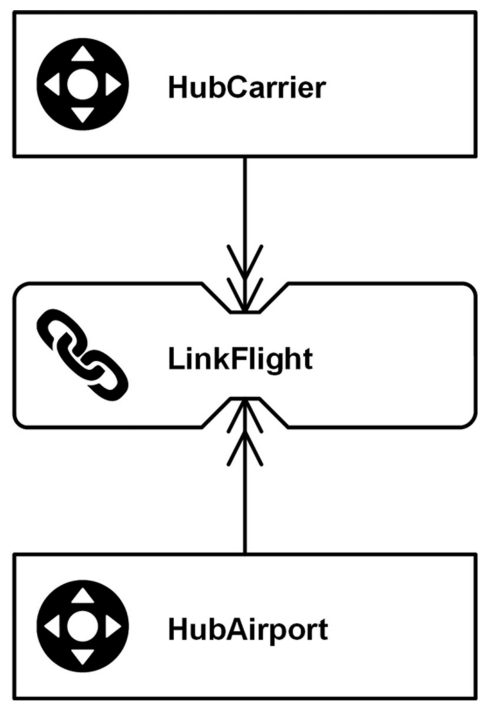
\includegraphics[scale=0.3]{../images/link.png}
	\caption{Link entiteit die 2 hub entiteiten met elkaar verbindt. \autocite{Linstedt2016}.}
	\label{fig:link}
\end{figure}

Ook bij links moeten er een aantal attributen aanwezig zijn:

\begin{itemize}
	\item \textbf{Hashkey (PK):} Als primaire sleutel van de entiteit worden alle business keys gehasht naar 1 sleutel.
	\item \textbf{LoadDate:} Datum/tijdstip wanneer de record is ingeladen
	\item \textbf{Record source:} Van welke databron is de record afkomstig?
	\item \textbf{Business key(s):} Alle business key(s) van de 2 gelinkte hub-entiteiten
\end{itemize} 

\subsubsection{Sattelieten}
In een satteliet worden alle gegevens gestockeerd dat een business object, relatie of transactie beschrijft. In de entiteit zelf is het belangrijk dat de historiek wordt bijgehouden. \autocite{Linstedt2016}

Bij een satteliet vinden we minstens volgende attributen terug:

\begin{itemize}
	\item \textbf{Parent Hashkey (PK):} Als primaire sleutel van de entiteit worden alle business keys gehasht naar 1 sleutel.
	\item \textbf{LoadDate:} Datum/tijdstip wanneer de record is ingeladen
	\item \textbf{Record source:} Van welke databron is de record afkomstig?
	\item \textbf{End load date:} Hierin wordt het moment geladen wanneer de entiteit niet meer gebruikt wordt (belangrijk voor het bewaren van de historiek).
\end{itemize} 

Een satteliet hoort bij een hub of een link. Een hub en een satteliet vormen een bepaald business object. 

\subsubsection{Data Vault schema}
Wanneer we zowel hubs, links als sattelieten samengieten in één schema, bekomen we een data vault. Wel zijn er nog enkele belangrijke opmerkingen:

\begin{itemize}
	\item Hubs mogen nooit rechtstreeks verbonden met elkaar, dit moet altijd gebeuren via een link (anders verliest het model zijn flexibiliteit).
	\item Sattelieten kunnen zowel met hubs als links verbonden worden.
	\item Hubs/links kunnen meerdere sattelieten hebben: deze staan meestal voor verschillende databronnen.
	\item Een satteliet kan maar verbonden worden met 1 hub of link. 
\end{itemize} 

\begin{figure}[h]
	\centering
	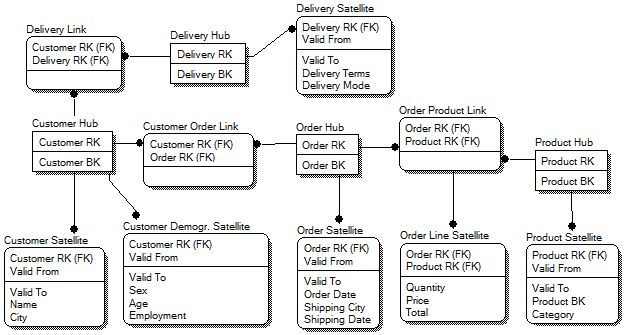
\includegraphics[scale=0.7]{../images/dvmodel.png}
	\caption{Een voorbeeld van een data vault model (Bukhantsov.org)}
	\label{fig:dvmod}
\end{figure}

Dit model heeft veel flexibiliteit te bieden. Enerzijds kan er gemakkelijk nieuwe hubs toevoegen door een nieuwe link te leggen. Ook kan er heel gemakkelijk een nieuwe gegevensbron toevoegen, dit wordt gedaan door een nieuwe satteliet toe te voegen aan een bestaande hub. 

\section{Rapporteringsomgevingen}
Inleiding enzoooooo

\subsection{Verschil tussen een measure en dimensie}
Lalalalalalallalala

\subsection{Rapporteringsomgevingen}
\label{sec:omgeving}
Inleiding enzoooooo

\subsubsection{SAP Analytics Cloud}
Lalalalalalallalala

\subsubsection{Power BI}
Lalalalalalallalala

\subsubsection{Andere omgevingen}
Naast de mogelijkheden die 2 grootmachten in de ERP-markt aanbieden, zijn er nog een aantal andere opties beschikbaar om rapporteringen visueel aantrekkelijk te maken. 






%%=============================================================================
%% Methodologie
%%=============================================================================

\chapter{Methodologie}
\label{ch:methodologie}

In Rapporteringsnood (hoofdstuk \ref{ch:rapporteringsnood}) wordt de te implementeren Key Performance Indicator (KPI) toegelicht. Er wordt in detail overlopen wat de KPI betekent en wat er exact moet berekend worden.

In Betekenis van de brondata (hoofdstuk \ref{ch:betekenisdata}) wordt de betekenis van de source data uitgeschreven zodat alle data duidelijk geïnterpreteerd kan worden.

Daara zal het onderzoek opgedeeld worden in twee onderdelen: het voorbereidende werk en het vergelijkend onderzoek. 

In het voorbereidende werk beschrijven we wat de benodigdheden zijn voor dit experiment en worden twee data warehouses stap voor stap opgebouwd. De ene data warehouse gebaseerd op het dimensioneel model, de andere data warehouse gebaseerd op Data Vault. Het gehele ETL-proces (\ref{sec:etl}) wordt neergepend in deze paper voor zowel Data Vault als voor het dimensioneel model. Hierdoor kan het experiment (indien gewenst) nagebootst worden. De gebruikte data-files zal als bijlage toegevoegd worden aan dit document.

In het vergelijkend onderzoek zal de onderzoeksvraag en deelvragen beantwoord worden. 

% Voeg hier je eigen hoofdstukken toe die de ``corpus'' van je bachelorproef
% vormen. De structuur en titels hangen af van je eigen onderzoek. Je kan bv.
% elke fase in je onderzoek in een apart hoofdstuk bespreken.

%\input{...}
%\input{...}
%...

%%=============================================================================
%% Conclusie
%%=============================================================================

\chapter{Conclusie}
\label{ch:conclusie}

%% TODO: Trek een duidelijke conclusie, in de vorm van een antwoord op de
%% onderzoeksvra(a)g(en). Wat was jouw bijdrage aan het onderzoeksdomein en
%% hoe biedt dit meerwaarde aan het vakgebied/doelgroep? Reflecteer kritisch
%% over het resultaat. Had je deze uitkomst verwacht? Zijn er zaken die nog
%% niet duidelijk zijn? Heeft het onderzoek geleid tot nieuwe vragen die
%% uitnodigen tot verder onderzoek?

Voor DHL Pharma Logistics werd gekozen om een data warehouse te ontwerpen aan de hand van de Data Vault methodologie. Was dit de juiste keuze? Was het dimensioneel model in hun project geen betere keuze? Wat wijst deze vergelijkende studie uit?

Het onderzoek wijst uit dat het dimensioneel model een betere keuze was voor het modelleren van de data voor DHL Pharma Logistics. Dit is bovendien ook het resultaat dat ik verwacht had.

Het dimensioneel model voert sneller leesresultaten uit in vergelijking met het Data Vault, dit omdat het Data Vault model meer relaties heeft. Hierdoor zullen veel meer joins moeten gebeuren wanneer alle data moet opgehaald worden. 

Bij de Data Vault methodologie wordt er meer informatie (Hash keys, informatie over extractie, ..) en tabellen opgeslagen in een databank. Dit zorgt ervoor dat de volumes van data enorm stijgen. Bijgevolg zal er dus een hogere kostprijs zijn om deze data te stockeren. Aangezien dit geen requirement is voor DHL Pharma Logistics, zou dit leiden naar een onnodige meerkost voor dit project.

De KPI's waarvoor een model moet opgesteld worden zijn gestandaardiseerd, en dienen niet flexibel te zijn. Indien de berekening voor de KPI's zouden gewijzigd worden, hoeven enkel sommige parameters uit het ETL-proces aangepast te worden en niet het datamodel zelf.

Het grote nadeel voor het implementeren van een project aan de hand van het dimensioneel model, is dat er niet kan gewerkt worden via de agile manier.

Er kan verder onderzoek verricht worden naar hoe het Data Vault model omspringt met NoSQL-data en big data in het algemeen. Is het een betere keuze om een Data Vault model te gebruiken bij big data modellen (aangezien Data Vault parallel inladen van data toelaat)? 

%%=============================================================================
%% Bijlagen
%%=============================================================================

\appendix

%%---------- Onderzoeksvoorstel -----------------------------------------------

\chapter{Onderzoeksvoorstel}

Het onderwerp van deze bachelorproef is gebaseerd op een onderzoeksvoorstel dat vooraf werd beoordeeld door de promotor. Dat voorstel is opgenomen in deze bijlage.

% Verwijzing naar het bestand met de inhoud van het onderzoeksvoorstel
%---------- Inleiding ---------------------------------------------------------

\section{Introductie} % The \section*{} command stops section numbering
\label{sec:introductie}

Wanneer het management in het bedrijf een strategische of tactische beslissing wil maken, is deze beslissing gebaseerd op data afkomstig uit verschillende databronnen. Daarom is er bij grote ondernemingen (en tegenwoordig ook bij KMO’s) nood aan een rapporteringssysteem. Voor het opstellen en onderhouden van datawarehouses wordt een bepaald budget voorzien. Relaties leggen tussen verschillende data is dan ook een grote uitdaging. Daarom is het dus belangrijk dat het model op de juiste manier ontworpen wordt om kosten te beperken wanneer men de datawarehouse wil onderhouden/uitbreiden. Hiervoor bestaan verschillende modelleertechnieken. In dit onderzoek worden enkel het Kimball dimensioneel modelleren en Data Vault 2.0 vergeleken. We proberen in dit onderzoek de volgende vraag te beantwoorden: \textbf{Waar zitten de verschillen bij het modelleren met Data Vault 2.0 en het dimensioneel modelleren?}

Ook zal er een antwoord trachten gevonden te worden op volgende deelvragen:

\begin{itemize}
	\item Zijn er verschillende manieren van aanpak mogelijk?
	\item Hoe flexibel/schaalbaar zijn beide systemen?
	\item Is er een verschil in performantie?
	\item Hoe verschillen de technieken naar onderhoud toe?
\end{itemize}

Bij DHL Pharma Logistics gebeurt het berekenen van de KPI's (Key Performance Indicators) nog altijd manueel. Zo worden de KPI's berekend via een rekenmachine en handmatig ingevoerd in een Excel-bestand. De informatie die nodig is om verschillende berekeningen te maken is afkomstig uit verschillende databronnen (mainframe, Cronos, Excel-sheets, ..). Dit neemt veel tijd in beslag, dus beslist de firma om een deel van de KPI's te automatiseren. Hiervoor zal een datawarehouse moeten opgezet worden. Deze zal gemodelleerd worden in Data Vault 2.0. Maar is dit wel de beste oplossing? Dit onderzoek zal uitwijzen of Data Vault 2.0 wel degelijk de beste oplossing is.
%---------- Stand van zaken ---------------------------------------------------

\section{Literatuurstudie}
\label{sec:state-of-the-art}
\subsection{Data Vault 2.0}
\subsubsection{Architectuur}
De architectuur van Data vault bestaat voornamelijk uit 3 lagen: De staging area, de raw data vault area en de Business vault. De staging area wordt gebruikt om alle data tijdelijk te stockeren. Deze wordt opgeslagen in de architectuur van het bronsysteem. Daarna wordt de data doorgezonden naar de volgende laag: de raw data vault. Hierbij wordt de architectuur omgevormd naar een data vault. Hierop worden dan data manipulaties gemaakt en wordt de data doorgezonden naar de volgende laag, de business vault. Data marts worden gecreëerd op de business vault \autocite{Linstedt2015}.

\begin{figure}[h]
	\centering
	\includegraphics[scale=0.345]{images/DVArchitectuur.png}
	\caption{Data Vault architectuur voorgesteld door \textcite{Stroobants2018}.}
	\label{fig:dvarch}
\end{figure}

\subsubsection{Entiteittype's}
Bij data vault wordt er een onderscheid gemaakt tussen 3 verschillende entiteiten: hub, link en satelliet. In een hub wordt een hash sleutel opgeslagen die gebaseerd is op de identifier van die entiteit en metadata (zoals de bron en wanneer de record is ingevoerd). Een link is entiteit die verantwoordelijk is om verschillende hubs met elkaar te verbinden. Hierin worden de hash sleutels van de verbonden entiteiten in opgeslagen. Satellieten kunnen verbonden worden met hubs en links. Deze bevatten de inhoudelijke data van de entiteit.  

\subsection{Dimensioneel modelleren}
\subsubsection{Architectuur}
Bij het dimensioneel modelleren via Kimbell is er 1 enkele laag, hierin worden alle operaties uitgevoerd (ETL: Extraction, Transaction en Load). De data wordt ingeladen in een ster-schema. Op deze laag worden dan data marts gebouwd. \autocite{Jukic2006}

\subsubsection{Entiteittype's}
Bij deze techniek bestaan er 2 entiteittype's: feit tabellen en dimensionele tabellen. De feit tabellen bevatten alle transactionele data, data waarop je eigenlijk berekeningen kan maken. Dimensionele tabellen bevatten meer informatie over de transactionele data.

% Voor literatuurverwijzingen zijn er twee belangrijke commando's:
% \autocite{KEY} => (Auteur, jaartal) Gebruik dit als de naam van de auteur
%   geen onderdeel is van de zin.
% \textcite{KEY} => Auteur (jaartal)  Gebruik dit als de auteursnaam wel een
%   functie heeft in de zin (bv. ``Uit onderzoek door Doll & Hill (1954) bleek
%   ...'')


%---------- Methodologie ------------------------------------------------------
\section{Methodologie}
\label{sec:methodologie}
Voor dit onderzoek zullen er twee datawarehouses opgezet worden in een SAP HANA-omgeving. De eerste datawarehouse zal gemodelleerd worden in Data Vault 2.0, de andere in een dimensioneel model. De SAP HANA omgeving is 'on-premise' die draait in een Microsoft Azure omgeving. Het modelleren zal deels gebeuren in Eclipse (die een remote-verbinding maakt met Azure) en deels via een web IDE voor HANA (Xsengine). Wanneer beide datawarehouses operationeel zijn, kan er gestart worden met de vergelijking. De datawarehouses zullen gebaseerd zijn op KPI's die gedefinieerd zijn bij DHL Pharma Logistics.

\subsection{Performatie}
Om de performantie van beide systemen te vergelijken, zullen er een aantal verschillende queries uitgevoerd worden op data marts gebaseerd op deze datawarehouses. Op basis van uitvoeringstijd kunnen we deze dan met elkaar vergelijken. Zo kunnen we te weten komen of er wel degelijk een verschil is tussen beide architecturen in performantie en hoe groot de verschillen zijn. 

\subsection{Audit}
Stel dat er op 2 verschillende databronnen klantengegevens opgeslagen wordt, zal er een keuze moeten gemaakt worden. Van welke bron haal ik mijn gegevens? Indien er verschillende problemen optreden met data, willen we graag kunnen onderzoeken waar het probleem zich heeft voorgedaan. Hiervoor voegen we META-data toe aan de data die ons verteld waar en wanneer de data werd opgehaald. 

\subsection{Schaalbaarheid}
Hoe wordt er omgegaan met grote hoeveelheden data in beide architecturen? Merken we hier een significant verschil? Zien we de uitvoeringstijden lineair/exponentieel stijgen? 

\subsection{Flexibiliteit}
De vereisten voor rapportering verandert vaak bij bedrijven. Soms moeten KPI's worden toegevoegd, soms moeten deze gewijzigd worden. Maar wat als er databronnen in het bedrijfsnetwerk toegevoegd? Hoe gemakkelijk kunnen deze wijzigingen gemaakt worden in beide architecturen? Dit zullen we onderzoeken door een nieuwe KPI toe te voegen aan het systeem. 
 


%---------- Verwachte resultaten ----------------------------------------------
\section{Verwachte resultaten}
\label{sec:verwachte_resultaten}

Op basis van het uitgevoerde onderzoek zullen we hiervan een resultaat kunnen opstellen. Ik verwacht dat beide technieken zijn voordelen en nadelen zullen hebben. Zo zal Data Vault 2.0 een modelleertechniek zijn die zeer flexibel is, maar dit zal ten koste gaan van de performantie. Het dimensionele model zal zo performanter zijn, maar weinig flexibiliteit bieden.

%---------- Verwachte conclusies ----------------------------------------------
\section{Verwachte conclusies}
\label{sec:verwachte_conclusies}

Aangezien Data Vault 2.0 veel flexibiliteit te bieden heeft, zal dit de beste oplossing zijn wanneer alle data verspreidt staat op verschillende systemen. Bij Data Vault 2.0 is het namelijk mogelijk gemakkelijk nieuwe databronnen toe te voegen in een datawarehouse. Maar wanneer men de de data marts wil ontwerpen, zal men nog steeds moeten gebruik maken van dimensioneel modelleren. Wanneer een bedrijf weinig databronnen heeft en deze weinig veranderen, is dimensioneel modelleren de betere oplossing. 

Voor DHL Pharma Logistics zal Data Vault 2.0 dan ook de beste oplossing zijn, aangezien hun data verspreidt staat over enkele systemen. Zo kunnen ze hun KPI's ook nog beter definiëren en makkelijker aanpassen in het systeem. 


%%---------- Andere bijlagen --------------------------------------------------
% TODO: Voeg hier eventuele andere bijlagen toe
%\input{...}

%%---------- Referentielijst --------------------------------------------------

\printbibliography[heading=bibintoc]
%\addcontentsline{toc}{chapter}{\textcolor{maincolor}{\IfLanguageName{dutch}{Bibliografie}{Bibliography}}}

\end{document}
